\documentclass{standalone}
\usepackage{tikz}
\usetikzlibrary{patterns, positioning}


\begin{document}
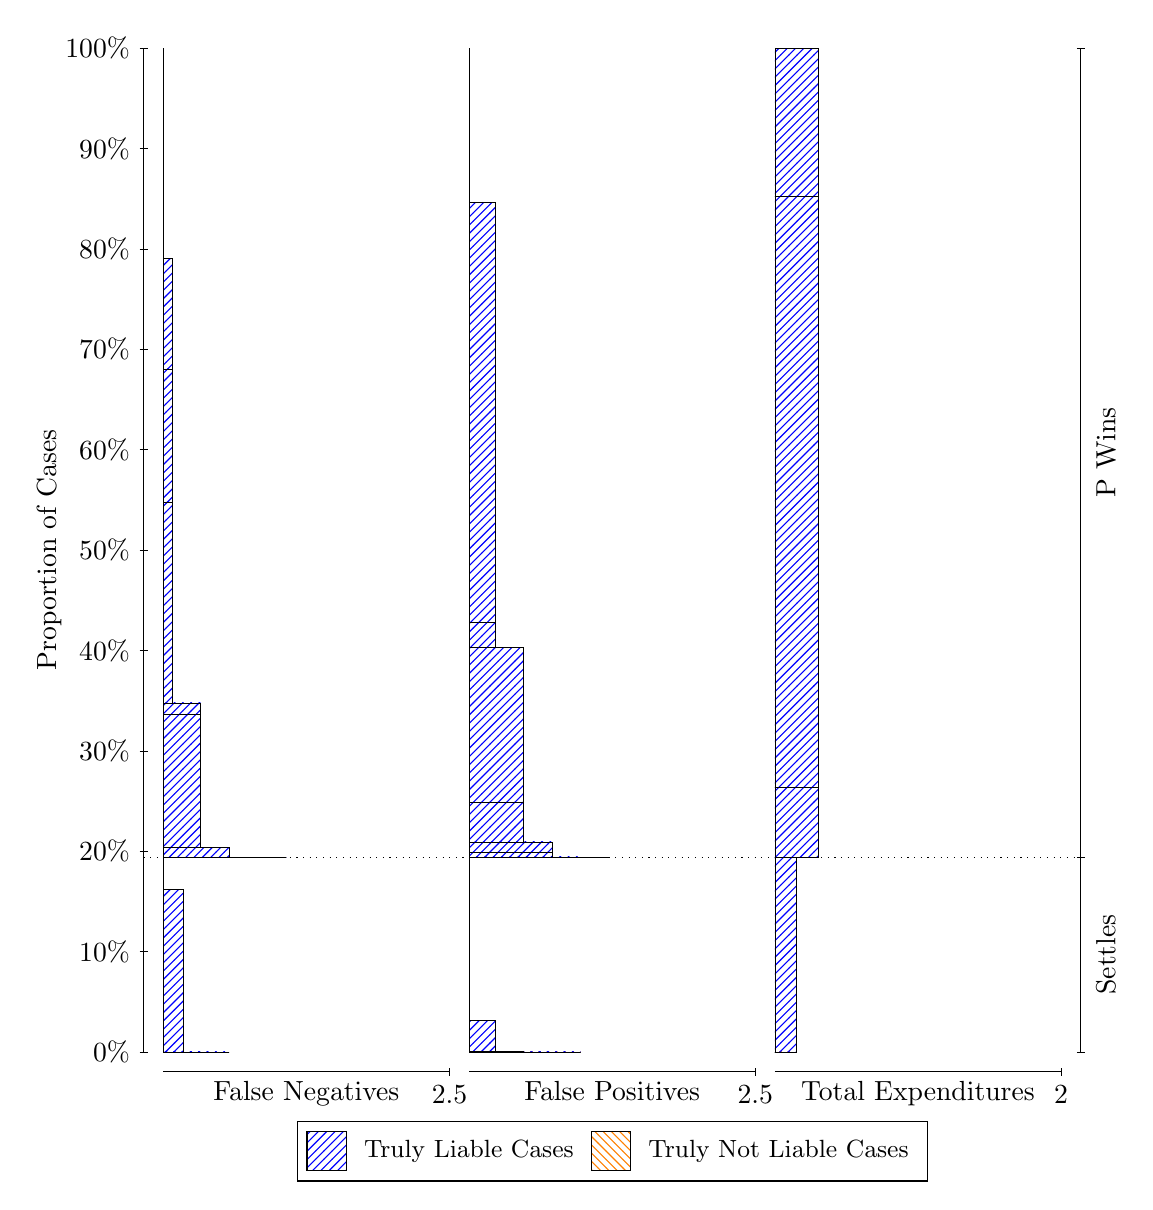
\begin{tikzpicture}
\draw[black, very thin] (1.5,1.75) -- (1.5,14.5);
\node[rotate=90, text=black, anchor=center] at (0.3, 8.125) {Proportion of Cases};
\draw[black, very thin] (1.45,1.75) -- (1.55,1.75);
\node[text=black, anchor=east] at (1.45, 1.75) {0\%};
\draw[black, very thin] (1.45,3.025) -- (1.55,3.025);
\node[text=black, anchor=east] at (1.45, 3.025) {10\%};
\draw[black, very thin] (1.45,4.3) -- (1.55,4.3);
\node[text=black, anchor=east] at (1.45, 4.3) {20\%};
\draw[black, very thin] (1.45,5.575) -- (1.55,5.575);
\node[text=black, anchor=east] at (1.45, 5.575) {30\%};
\draw[black, very thin] (1.45,6.85) -- (1.55,6.85);
\node[text=black, anchor=east] at (1.45, 6.85) {40\%};
\draw[black, very thin] (1.45,8.125) -- (1.55,8.125);
\node[text=black, anchor=east] at (1.45, 8.125) {50\%};
\draw[black, very thin] (1.45,9.4) -- (1.55,9.4);
\node[text=black, anchor=east] at (1.45, 9.4) {60\%};
\draw[black, very thin] (1.45,10.675) -- (1.55,10.675);
\node[text=black, anchor=east] at (1.45, 10.675) {70\%};
\draw[black, very thin] (1.45,11.95) -- (1.55,11.95);
\node[text=black, anchor=east] at (1.45, 11.95) {80\%};
\draw[black, very thin] (1.45,13.225) -- (1.55,13.225);
\node[text=black, anchor=east] at (1.45, 13.225) {90\%};
\draw[black, very thin] (1.45,14.5) -- (1.55,14.5);
\node[text=black, anchor=east] at (1.45, 14.5) {100\%};

\draw[black, very thin] (13.4,1.75) -- (13.4,14.5);
\draw[black, very thin] (13.35,1.75) -- (13.45,1.75);
\node[anchor=west] at (13.35, 1.75) {};
\draw[black, very thin] (13.35,4.2246) -- (13.45,4.2246);
\node[anchor=west] at (13.35, 4.2246) {};
\draw[black, very thin] (13.35,14.5) -- (13.45,14.5);
\node[anchor=west] at (13.35, 14.5) {};

\draw[black, very thin, pattern color=blue, pattern=north east lines] (1.75,1.75) rectangle (2.5857,1.75);
\draw[black, very thin, pattern color=blue, pattern=north east lines] (1.75,1.75) rectangle (2.295,1.75);
\draw[black, very thin, pattern color=blue, pattern=north east lines] (1.75,1.75) rectangle (2.2223,1.75);
\draw[black, very thin, pattern color=blue, pattern=north east lines] (1.75,1.75) rectangle (2.0043,3.8191);
\draw[black, very thin, pattern color=blue, pattern=north east lines] (1.75,3.8191) rectangle (1.9317,3.8191);
\draw[black, very thin, pattern color=blue, pattern=north east lines] (1.75,3.8191) rectangle (1.859,3.8193);
\draw[black, very thin, pattern color=orange, pattern=north west lines] (1.75,3.8193) rectangle (1.75,3.8193);
\draw[black, very thin, pattern color=blue, pattern=north east lines] (1.75,3.8193) rectangle (1.75,4.2246);
\draw[black, very thin, pattern color=blue, pattern=north east lines] (1.75,4.2246) rectangle (3.3123,4.2246);
\draw[black, very thin, pattern color=blue, pattern=north east lines] (1.75,4.2246) rectangle (2.949,4.2258);
\draw[black, very thin, pattern color=blue, pattern=north east lines] (1.75,4.2258) rectangle (2.5857,4.3461);
\draw[black, very thin, pattern color=blue, pattern=north east lines] (1.75,4.3461) rectangle (2.2223,6.0361);
\draw[black, very thin, pattern color=blue, pattern=north east lines] (1.75,6.0361) rectangle (2.2223,6.1839);
\draw[black, very thin, pattern color=blue, pattern=north east lines] (1.75,6.1839) rectangle (1.859,8.7371);
\draw[black, very thin, pattern color=blue, pattern=north east lines] (1.75,8.7371) rectangle (1.859,10.426);
\draw[black, very thin, pattern color=blue, pattern=north east lines] (1.75,10.426) rectangle (1.859,11.832);
\draw[black, very thin, pattern color=orange, pattern=north west lines] (1.75,11.832) rectangle (1.75,11.832);
\draw[black, very thin, pattern color=blue, pattern=north east lines] (1.75,11.832) rectangle (1.75,14.5);
\draw[black, very thin, pattern color=orange, pattern=north west lines] (5.6333,1.75) rectangle (7.0503,1.75);
\draw[black, very thin, pattern color=blue, pattern=north east lines] (5.6333,1.75) rectangle (7.0503,1.75);
\draw[black, very thin, pattern color=orange, pattern=north west lines] (5.6333,1.75) rectangle (6.7597,1.75);
\draw[black, very thin, pattern color=blue, pattern=north east lines] (5.6333,1.75) rectangle (6.7597,1.75);
\draw[black, very thin, pattern color=blue, pattern=north east lines] (5.6333,1.75) rectangle (6.687,1.75);
\draw[black, very thin, pattern color=orange, pattern=north west lines] (5.6333,1.75) rectangle (6.469,1.75);
\draw[black, very thin, pattern color=blue, pattern=north east lines] (5.6333,1.75) rectangle (6.469,1.75);
\draw[black, very thin, pattern color=blue, pattern=north east lines] (5.6333,1.75) rectangle (6.3963,1.75);
\draw[black, very thin, pattern color=blue, pattern=north east lines] (5.6333,1.75) rectangle (6.3237,1.7535);
\draw[black, very thin, pattern color=blue, pattern=north east lines] (5.6333,1.7535) rectangle (6.1057,1.7536);
\draw[black, very thin, pattern color=blue, pattern=north east lines] (5.6333,1.7536) rectangle (6.033,1.7536);
\draw[black, very thin, pattern color=blue, pattern=north east lines] (5.6333,1.7536) rectangle (5.9603,2.1553);
\draw[black, very thin, pattern color=blue, pattern=north east lines] (5.6333,2.1553) rectangle (5.7423,2.1555);
\draw[black, very thin, pattern color=blue, pattern=north east lines] (5.6333,2.1555) rectangle (5.6697,2.1555);
\draw[black, very thin, pattern color=blue, pattern=north east lines] (5.6333,2.1555) rectangle (5.6333,4.2246);
\draw[black, very thin, pattern color=orange, pattern=north west lines] (5.6333,4.2246) rectangle (7.4137,4.2246);
\draw[black, very thin, pattern color=blue, pattern=north east lines] (5.6333,4.2246) rectangle (7.4137,4.2246);
\draw[black, very thin, pattern color=blue, pattern=north east lines] (5.6333,4.2246) rectangle (7.0503,4.2257);
\draw[black, very thin, pattern color=orange, pattern=north west lines] (5.6333,4.2257) rectangle (7.0503,4.2257);
\draw[black, very thin, pattern color=blue, pattern=north east lines] (5.6333,4.2257) rectangle (7.0503,4.2272);
\draw[black, very thin, pattern color=blue, pattern=north east lines] (5.6333,4.2272) rectangle (6.687,4.2841);
\draw[black, very thin, pattern color=orange, pattern=north west lines] (5.6333,4.2841) rectangle (6.687,4.2841);
\draw[black, very thin, pattern color=blue, pattern=north east lines] (5.6333,4.2841) rectangle (6.687,4.4184);
\draw[black, very thin, pattern color=blue, pattern=north east lines] (5.6333,4.4184) rectangle (6.3237,4.9235);
\draw[black, very thin, pattern color=orange, pattern=north west lines] (5.6333,4.9235) rectangle (6.3237,4.9235);
\draw[black, very thin, pattern color=blue, pattern=north east lines] (5.6333,4.9235) rectangle (6.3237,6.8922);
\draw[black, very thin, pattern color=blue, pattern=north east lines] (5.6333,6.8922) rectangle (5.9603,7.2106);
\draw[black, very thin, pattern color=orange, pattern=north west lines] (5.6333,7.2106) rectangle (5.9603,7.2106);
\draw[black, very thin, pattern color=blue, pattern=north east lines] (5.6333,7.2106) rectangle (5.9603,12.541);
\draw[black, very thin, pattern color=blue, pattern=north east lines] (5.6333,12.541) rectangle (5.6333,14.5);
\draw[black, very thin, pattern color=orange, pattern=north west lines] (9.5167,1.75) rectangle (9.7892,1.75);
\draw[black, very thin, pattern color=blue, pattern=north east lines] (9.5167,1.75) rectangle (9.7892,1.7504);
\draw[black, very thin, pattern color=orange, pattern=north west lines] (9.5167,1.7504) rectangle (9.7892,1.7504);
\draw[black, very thin, pattern color=blue, pattern=north east lines] (9.5167,1.7504) rectangle (9.7892,4.2246);
\draw[black, very thin, pattern color=orange, pattern=north west lines] (9.5167,4.2246) rectangle (10.062,4.2246);
\draw[black, very thin, pattern color=blue, pattern=north east lines] (9.5167,4.2246) rectangle (10.062,5.1061);
\draw[black, very thin, pattern color=orange, pattern=north west lines] (9.5167,5.1061) rectangle (10.062,5.1061);
\draw[black, very thin, pattern color=blue, pattern=north east lines] (9.5167,5.1061) rectangle (10.062,12.619);
\draw[black, very thin, pattern color=orange, pattern=north west lines] (9.5167,12.619) rectangle (10.062,12.619);
\draw[black, very thin, pattern color=blue, pattern=north east lines] (9.5167,12.619) rectangle (10.062,14.5);
\draw[black, dotted] (1.5,4.2246) -- (13.4,4.2246);
\draw[black, very thin] (1.75,1.5) -- (5.3833,1.5);
\node[text=black, anchor=north] at (3.5667, 1.5) {False Negatives};
\draw[black, very thin] (5.3833,1.45) -- (5.3833,1.55);
\node[text=black, anchor=north] at (5.3833, 1.45) {2.5};

\draw[black, very thin] (5.6333,1.5) -- (9.2667,1.5);
\node[text=black, anchor=north] at (7.45, 1.5) {False Positives};
\draw[black, very thin] (9.2667,1.45) -- (9.2667,1.55);
\node[text=black, anchor=north] at (9.2667, 1.45) {2.5};

\draw[black, very thin] (9.5167,1.5) -- (13.15,1.5);
\node[text=black, anchor=north] at (11.333, 1.5) {Total Expenditures};
\draw[black, very thin] (13.15,1.45) -- (13.15,1.55);
\node[text=black, anchor=north] at (13.15, 1.45) {2};

\node[text=black, centered, rotate=90] at (13.72, 2.9873) {Settles};
\node[text=black, centered, rotate=90] at (13.72, 9.3623) {P Wins};

\draw (7.449999999999999,1.5) node[draw=none] (baseCoordinate) {};
\begin{scope}[align=center]
        \matrix[scale=0.5, draw=black, below=0.5cm of baseCoordinate, nodes={draw}, column sep=0.1cm]{
            \node[rectangle, draw, minimum width=0.5cm, minimum height=0.5cm, pattern color=blue, pattern=north east lines] {}; &
            \node[draw=none, font=\small, text=black] (B) {Truly Liable Cases}; &
            \node[rectangle, draw, minimum width=0.5cm, minimum height=0.5cm, pattern color=orange, pattern=north west lines] {}; &
            \node[draw=none, font=\small, text=black] (B) {Truly Not Liable Cases}; \\
            };
\end{scope}

\end{tikzpicture}
\end{document}